
\begin{figure}[ht]
    \centering
    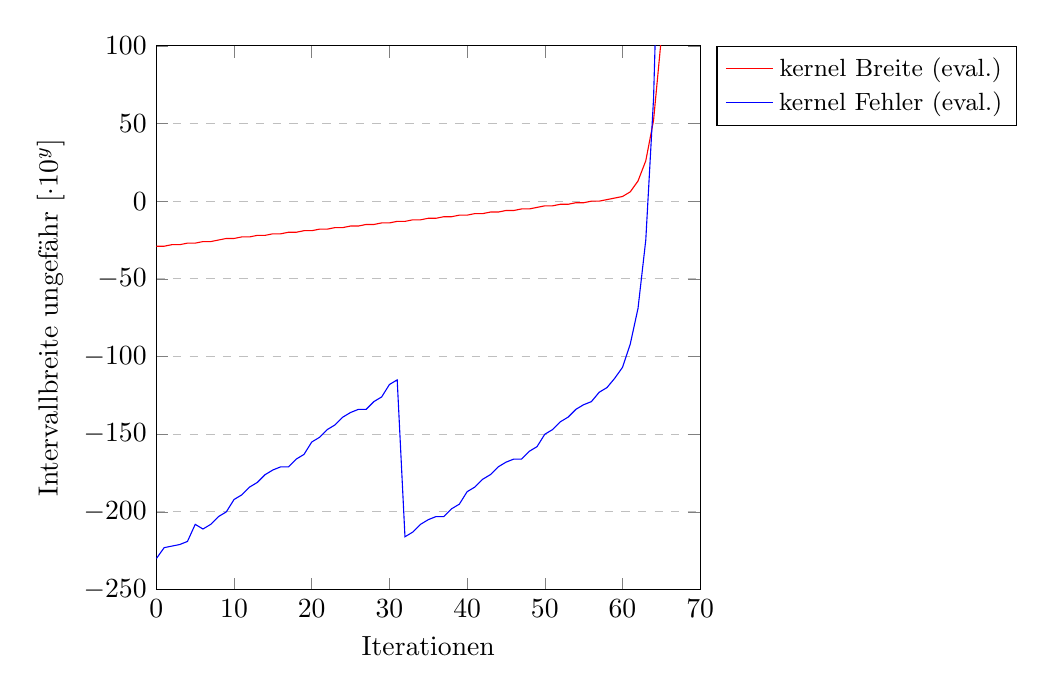
\begin{tikzpicture}
    \begin{axis}[
        width=0.7\textwidth,
        height=0.7\textwidth,
        xlabel={Iterationen},
        ylabel={Intervallbreite ungefähr $[\cdot 10^y ]$},
        legend pos=north west,
        xmin=0,xmax=70,
        ymax=100,ymin=-250,
        ymajorgrids=true,
        grid style=dashed,
        legend pos=outer north east,
        cycle list name=color list
    ]
    
    \addplot
        coordinates {
 (0,-29)
 (1,-29)
 (2,-28)
 (3,-28)
 (4,-27)
 (5,-27)
 (6,-26)
 (7,-26)
 (8,-25)
 (9,-24)
 (10,-24)
 (11,-23)
 (12,-23)
 (13,-22)
 (14,-22)
 (15,-21)
 (16,-21)
 (17,-20)
 (18,-20)
 (19,-19)
 (20,-19)
 (21,-18)
 (22,-18)
 (23,-17)
 (24,-17)
 (25,-16)
 (26,-16)
 (27,-15)
 (28,-15)
 (29,-14)
 (30,-14)
 (31,-13)
 (32,-13)
 (33,-12)
 (34,-12)
 (35,-11)
 (36,-11)
 (37,-10)
 (38,-10)
 (39,-9)
 (40,-9)
 (41,-8)
 (42,-8)
 (43,-7)
 (44,-7)
 (45,-6)
 (46,-6)
 (47,-5)
 (48,-5)
 (49,-4)
 (50,-3)
 (51,-3)
 (52,-2)
 (53,-2)
 (54,-1)
 (55,-1)
 (56,0)
 (57,0)
 (58,01)
 (59,02)
 (60,03)
 (61,06)
 (62,013)
 (63,026)
 (64,052)
 (65,0105)
        };
        \addlegendentry{\small{kernel Breite (eval.)}}
    
    \addplot
        coordinates {
  (0,-230)
 (1,-223)
 (2,-222)
 (3,-221)
 (4,-219)
 (5,-208)
 (6,-211)
 (7,-208)
 (8,-203)
 (9,-200)
 (10,-192)
 (11,-189)
 (12,-184)
 (13,-181)
 (14,-176)
 (15,-173)
 (16,-171)
 (17,-171)
 (18,-166)
 (19,-163)
 (20,-155)
 (21,-152)
 (22,-147)
 (23,-144)
 (24,-139)
 (25,-136)
 (26,-134)
 (27,-134)
 (28,-129)
 (29,-126)
 (30,-118)
 (31,-115)
 (32,-216)
 (33,-213)
 (34,-208)
 (35,-205)
 (36,-203)
 (37,-203)
 (38,-198)
 (39,-195)
 (40,-187)
 (41,-184)
 (42,-179)
 (43,-176)
 (44,-171)
 (45,-168)
 (46,-166)
 (47,-166)
 (48,-161)
 (49,-158)
 (50,-150)
 (51,-147)
 (52,-142)
 (53,-139)
 (54,-134)
 (55,-131)
 (56,-129)
 (57,-123)
 (58,-120)
 (59,-114)
 (60,-107)
 (61,-92)
 (62,-69)
 (63,-25)
 (64,66)
 (65,241)
        };
        \addlegendentry{\small{kernel Fehler (eval.)}}
      
    
    \end{axis}
    \end{tikzpicture}
    \caption{$x_0 = [0.5 \pm \varepsilon]$}
    \label{fig:tm6}
\end{figure}